\documentclass[aspectratio=169,11pt]{beamer}

% ==========================================================
% 1. PACKAGES AND FONTS
% ==========================================================

\usepackage{iftex}

\ifPDFTeX
  \usepackage[T1]{fontenc}
  \usepackage{tgheros}
  \renewcommand{\familydefault}{\sfdefault}
\else
  \usepackage{fontspec}
  \setsansfont{TeX Gyre Heros}
\fi

\usepackage{graphicx}
\usepackage{booktabs}
\usepackage{tabularx}
\usepackage{ragged2e}
\usepackage{tikz}

% ==========================================================
% 2. FILE NAMES — EDIT HERE
% All figures are PNG.
% ==========================================================

% Descriptive figures
\newcommand{\FigLandscape}{fwa.png}
\newcommand{\FigSetup}{employee_fwa_setup.png}
\newcommand{\FigAwareness}{fwa_awareness.png}
\newcommand{\FigRequests}{formal_requests_outcomes.png}

% DCE and overall conditional-logit results
\newcommand{\FigDCEExample}{dce_example.png}
\newcommand{\FigEmployeeWTP}{employee_wtp_main.png}
\newcommand{\FigEmployerWTP}{employer_wtp_main.png}
\newcommand{\FigGap}{wtp_gap_employee_employer.png}

% Employee heterogeneity:
% Re-export selected attributes with axes and legends retained.
\newcommand{\FigGenderRemote}{employee_gender_remote.png}
\newcommand{\FigAgeSchedule}{employee_age_schedule.png}

% Employer constraints and concerns
\newcommand{\FigPresence}{employer_physical.png}
\newcommand{\FigConcerns}{employer_concern.png}

% Current practice:
% Employee main figure: compressed workweek and part-time.
% Full employee figure goes in the appendix.
\newcommand{\FigEmployeePractice}{employee_current_selected.png}
\newcommand{\FigEmployerPractice}{employer_current_wfh.png}

\newcommand{\StudyName}{SMU--SNEF FWA Study}

% Headline numbers used in more than one place
\newcommand{\PolicyShare}{66.0}   % employers with a formal written FWA policy (%)

% ==========================================================
% 3. COLOURS
% Employee (blue) and Employer (orange) are reserved for
% the two survey samples; Navy / Muted are neutral.
% ==========================================================

\definecolor{Navy}{HTML}{304A75}
\definecolor{Employee}{HTML}{6D82A0}
\definecolor{EmployeeLight}{HTML}{BED7ED}
\definecolor{Employer}{HTML}{B57A50}
\definecolor{EmployerLight}{HTML}{F2D8B8}

\definecolor{Ink}{HTML}{252B33}
\definecolor{Muted}{HTML}{636B75}
\definecolor{Rule}{HTML}{DFE3E8}
\definecolor{Soft}{HTML}{F5F7FA}

% ==========================================================
% 4. BEAMER STYLE
% A 16:9 beamer page is 16cm x 9cm, so sizes below are
% chosen against that page (not against A4).
% ==========================================================

\usetheme{default}

\setbeamertemplate{navigation symbols}{}
\setbeamertemplate{headline}{}

\setbeamercolor{normal text}{fg=Ink,bg=white}
\setbeamercolor{frametitle}{fg=Navy,bg=white}
\setbeamercolor{structure}{fg=Navy}
\setbeamercolor{itemize item}{fg=Navy}
\setbeamercolor{enumerate item}{fg=Navy}

\setbeamersize{
  text margin left=0.65cm,
  text margin right=0.65cm
}

\setbeamerfont{frametitle}{
  size=\fontsize{18}{21}\selectfont,
  series=\bfseries
}

\setbeamerfont{itemize/enumerate body}{
  size=\fontsize{12}{15}\selectfont
}

\setbeamertemplate{itemize item}{\small$\bullet$}

% ----------------------------------------------------------
% Section kicker shown above every frame title.
% Set it between frames with \SetPart{...}; it keeps
% titles at the same height on every slide and tells the
% audience which research question a slide answers.
% ----------------------------------------------------------

\def\CurrentPart{}
\newcommand{\SetPart}[1]{\gdef\CurrentPart{#1}}

\setbeamertemplate{frametitle}{%
  \vspace{0.12cm}
  \begin{beamercolorbox}[wd=\textwidth,sep=0pt]{frametitle}
    \ifx\CurrentPart\empty\else
      {\color{Muted}\fontsize{7.5}{9}\selectfont\bfseries
       \MakeUppercase{\CurrentPart}\par}
      \vspace{0.05cm}
    \fi
    \usebeamerfont{frametitle}\insertframetitle\par
  \end{beamercolorbox}
  \vspace{0.12cm}
}

% ==========================================================
% 5. FOOTER
% Cover unnumbered; main body 1--15; appendix A1, A2, ...
% The switch to A-numbering is made just before the
% appendix divider (see \StartAppendix below).
% ==========================================================

\newif\ifappendixslides
\appendixslidesfalse

\newcounter{mainend}

\newcommand{\StartAppendix}{%
  \setcounter{mainend}{\value{framenumber}}%
  \global\appendixslidestrue
}

\newcommand{\DisplayPage}{%
  \ifappendixslides
    A\the\numexpr\value{framenumber}-\value{mainend}\relax
  \else
    \insertframenumber
  \fi
}

\setbeamertemplate{footline}{%
  \leavevmode%
  \hbox{%
    \begin{beamercolorbox}[
      wd=\paperwidth,
      ht=0.25cm,
      dp=0.12cm,
      leftskip=0.65cm,
      rightskip=0.65cm
    ]{normal text}%
      \color{Muted}%
      \fontsize{7.5}{9}\selectfont
      \StudyName
      \ifappendixslides\enspace|\enspace Appendix\fi
      \hfill
      \DisplayPage
    \end{beamercolorbox}%
  }%
}

% ==========================================================
% 6. TEXT ELEMENTS
% ==========================================================

\newcommand{\PanelTitle}[2]{%
  {\color{#1}\fontsize{12.5}{15}\selectfont
   \bfseries #2\par}
  \vspace{0.06cm}
}

\newcommand{\Subline}[1]{%
  {\color{Muted}\fontsize{10}{12.5}\selectfont
   \RaggedRight #1\par}
  \vspace{0.10cm}
}

\newcommand{\SlideNote}[1]{%
  \par\vspace{0.07cm}
  {\color{Muted}\fontsize{7.5}{9}\selectfont
   \RaggedRight #1\par}
}

\newcommand{\Takeaway}[1]{%
  \par\vspace{0.08cm}
  {\color{Rule}\hrule height 0.5pt}
  \vspace{0.08cm}
  {\color{Navy}\fontsize{11}{13.5}\selectfont\bfseries
   \hyphenpenalty=10000\exhyphenpenalty=10000
   \raggedright #1\par}
}

\newcommand{\EditText}[1]{%
  {\color{Muted}\fontsize{11}{14}\selectfont
   \RaggedRight #1\par}
}

% ==========================================================
% 7. FIXED-HEIGHT FIGURE BOX
%
% \FitFigure[trim]{file}{height}{placeholder}
% trim = LEFT BOTTOM RIGHT TOP
% ==========================================================

\newcommand{\FitFigure}[4][0pt 0pt 0pt 0pt]{%
  \par\noindent
  \begin{minipage}[c][#3][c]{\linewidth}
    \centering
    \IfFileExists{#2}{%
      \includegraphics[
        width=\linewidth,
        height=#3,
        keepaspectratio,
        trim={#1},
        clip
      ]{#2}%
    }{%
      \begingroup
      \setlength{\fboxsep}{0pt}
      \fcolorbox{Rule}{Soft}{%
        \parbox[c][\dimexpr#3-2\fboxrule\relax][c]
          {\dimexpr\linewidth-2\fboxrule\relax}{%
          \centering
          \color{Muted}
          \fontsize{10}{13}\selectfont
          #4\par
          \vspace{0.12cm}
          {\fontsize{8.5}{10}\selectfont
           PNG figure placeholder\par}
        }%
      }%
      \endgroup
    }%
  \end{minipage}
  \par
}

% ==========================================================
% 8. PROPORTIONAL PNG CROPPING
%
% \CropPNG{file}{left}{bottom}{right}{top}{max height}
% 0.05 = crop 5% of original width/height.
% ==========================================================

\newsavebox{\PNGMeasure}
\newlength{\PNGLeft}
\newlength{\PNGBottom}
\newlength{\PNGRight}
\newlength{\PNGTop}

\newcommand{\CropPNG}[6]{%
  \par\noindent
  \begingroup
  \IfFileExists{#1}{%
    \sbox{\PNGMeasure}{\includegraphics{#1}}%
    \setlength{\PNGLeft}{#2\wd\PNGMeasure}%
    \setlength{\PNGBottom}{#3\ht\PNGMeasure}%
    \setlength{\PNGRight}{#4\wd\PNGMeasure}%
    \setlength{\PNGTop}{#5\ht\PNGMeasure}%
    \edef\PNGDraw{%
      \noexpand\includegraphics[
        trim={\the\PNGLeft\space\the\PNGBottom\space\the\PNGRight\space\the\PNGTop},
        clip,
        width=\the\linewidth,
        height=#6,
        keepaspectratio
      ]{#1}%
    }%
    \makebox[\linewidth][c]{\PNGDraw}%
  }{%
    \FitFigure{#1}{#6}{Upload the PNG figure}%
  }%
  \par
  \endgroup
}

% Appendix figure template (no notes, so the figure can
% use almost the full body height)
\newcommand{\AppendixFigure}[3]{%
  \begin{frame}[t]{#1}
    \FitFigure{#2}{6.45cm}{#3}
  \end{frame}
}

\begin{document}

% ==========================================================
% COVER (unnumbered)
% ==========================================================

\begin{frame}[plain,noframenumbering]

\vspace*{1.35cm}

{\color{Navy}\fontsize{28}{33}\selectfont\bfseries
Measuring the Flexibility Gap\par}

\vspace{0.30cm}

{\color{Employer}\rule{1.6cm}{2pt}\par}

\vspace{0.30cm}

{\color{Ink}\fontsize{14}{18}\selectfont
Employer and Employee Valuations of\\
Flexible Work Arrangements in Singapore\par}

\vfill

{\color{Muted}\fontsize{12}{15}\selectfont
\StudyName\par}

\vspace{0.12cm}

{\color{Muted}\fontsize{10.5}{14}\selectfont
[Presenters]\enspace|\enspace[Date]\par}

\vspace{0.45cm}

\end{frame}

% ==========================================================
% 1 — STUDY OVERVIEW
% ==========================================================

\SetPart{Introduction}

\begin{frame}[t]{Study Overview}

\vspace{0.10cm}

\begin{columns}[T,onlytextwidth]

\begin{column}{0.60\textwidth}

\PanelTitle{Navy}{Research questions}

\begin{enumerate}
  \setlength{\itemsep}{0.32cm}
  \item How are FWAs currently accessed and used?
  \item Which arrangements do employees and employers value,
        and by how much?
  \item What support could help increase effective FWA use?
\end{enumerate}

\end{column}

\begin{column}{0.33\textwidth}

\PanelTitle{Employee}{Employee survey}

{\color{Employee}\fontsize{30}{34}\selectfont
\bfseries 1,020\par}

\Subline{respondents}

\vspace{0.30cm}

\PanelTitle{Employer}{Employer survey}

{\color{Employer}\fontsize{30}{34}\selectfont
\bfseries 303\par}

\Subline{respondents}

\end{column}

\end{columns}

\vfill

\SlideNote{
Parallel online surveys of employees and employers, each with a
discrete choice experiment (DCE). Fieldwork: [dates].
Current-employment descriptives use 1,004 employee respondents.
Employee and employer samples are separate and unmatched.
}

\end{frame}

% ==========================================================
% PART 1 — ACCESS AND USE (RQ1)
% ==========================================================

\SetPart{1\enspace Access and use}

% ----------------------------------------------------------
% 2 — FWA LANDSCAPE
% ----------------------------------------------------------

\begin{frame}[t]{FWA Landscape}

% Remove the internal title; retain legend and notes.
\CropPNG{\FigLandscape}
  {0}{0}{0}{0.09}
  {5.60cm}

\vfill

\Takeaway{
[One-sentence takeaway on current FWA availability and use.]
}

\end{frame}

% ----------------------------------------------------------
% 3 — POLICIES AND PATHWAYS
% ----------------------------------------------------------

\begin{frame}[t]{Policies and Pathways}

\begin{columns}[T,onlytextwidth]

\begin{column}{0.64\textwidth}

\PanelTitle{Employee}{Employees}
\Subline{How current FWA was established}

\CropPNG{\FigSetup}
  {0.035}{0.12}{0.025}{0.15}
  {4.30cm}

\end{column}

\begin{column}{0.30\textwidth}

\PanelTitle{Employer}{Employers}
\Subline{Formal written FWA policy}

\vspace{0.45cm}

{\centering

  {\color{Employer}
   \fontsize{36}{40}\selectfont\bfseries
   \PolicyShare\%\par}

  \vspace{0.14cm}

  {\fontsize{11}{14}\selectfont
   have a formal written\\
   FWA policy\par}

}

\vspace{0.40cm}

% Bar is drawn from \PolicyShare, so it updates with the number.
{\centering
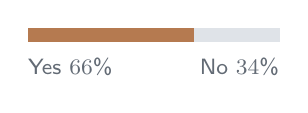
\begin{tikzpicture}[x=1cm,y=1cm]

  \pgfmathsetmacro{\BarYes}{3.2*\PolicyShare/100}
  \pgfmathsetmacro{\BarNoShare}{100-\PolicyShare}

  \fill[Employer]
    (0,0) rectangle (\BarYes,0.18);

  \fill[Rule]
    (\BarYes,0) rectangle (3.20,0.18);

  \node[
    anchor=north west,
    inner xsep=0pt,
    font=\fontsize{8.5}{10}\selectfont,
    text=Muted
  ] at (0,-0.08) {Yes \pgfmathprintnumber[fixed,precision=0]{\PolicyShare}\%};

  \node[
    anchor=north east,
    inner xsep=0pt,
    font=\fontsize{8.5}{10}\selectfont,
    text=Muted
  ] at (3.20,-0.08) {No \pgfmathprintnumber[fixed,precision=0]{\BarNoShare}\%};

\end{tikzpicture}
\par}

\end{column}

\end{columns}

\vfill

\Takeaway{
[One-sentence takeaway on formal policies versus informal pathways.]
}

\SlideNote{
Employee base: N=869; employed respondents selecting neither
``None'' nor ``Don't know'' in the original availability question.
Employer base: N=303. Samples are separate and unmatched.
}

\end{frame}

% ----------------------------------------------------------
% 4 — AWARENESS
% ----------------------------------------------------------

\begin{frame}[t]{TG-FWAR Awareness}

\CropPNG{\FigAwareness}
  {0.01}{0.09}{0.01}{0.11}
  {4.95cm}

\vfill

\Takeaway{
[One-sentence takeaway on how familiar each side is with TG-FWAR.]
}

\SlideNote{
Bases: currently employed employees, N=1,004; employers, N=303.
Familiarity is self-reported. Samples are separate and unmatched.
}

\end{frame}

% ----------------------------------------------------------
% 5 — REQUESTS AND OUTCOMES
% ----------------------------------------------------------

\begin{frame}[t]{Requests and Outcomes}

\Subline{Formal FWA requests since TG-FWAR took effect}

\begin{columns}[T,onlytextwidth]

\begin{column}{0.48\textwidth}

\PanelTitle{Employee}{Employees}

% Retain bottom outcome labels.
\CropPNG{\FigRequests}
  {0.025}{0.12}{0.515}{0.23}
  {3.40cm}

\end{column}

\begin{column}{0.48\textwidth}

\PanelTitle{Employer}{Employers}

\CropPNG{\FigRequests}
  {0.525}{0.12}{0.025}{0.23}
  {3.40cm}

\end{column}

\end{columns}

\vfill

\Takeaway{
[One-sentence takeaway on request rates and approval.]
}

\SlideNote{
Request questions were shown only to respondents who had heard of
TG-FWAR (employees also had to be currently employed).
Request bases: employees N=832; employers N=280.
Outcome bases: applicants N=547; receiving employers N=154.
Employee outcomes concern individual requests; employer outcomes
concern within-firm approval shares
(all or most=60--100\%; some or about half=10--59\%;
few or none=0--9\%). Samples are separate and unmatched.
}

\end{frame}

% ==========================================================
% PART 2 — VALUATIONS (RQ2)
% ==========================================================

\SetPart{2\enspace Valuations}

% ----------------------------------------------------------
% 6 — THE CHOICE EXPERIMENT
% ----------------------------------------------------------

\begin{frame}[t]{The Choice Experiment}

\begin{columns}[T,onlytextwidth]

\begin{column}{0.60\textwidth}

\PanelTitle{Navy}{An example choice}

\FitFigure{\FigDCEExample}{4.60cm}
  {Insert one readable DCE choice task}

\end{column}

\begin{column}{0.36\textwidth}

\PanelTitle{Navy}{How it works}

\setbeamerfont{itemize/enumerate body}{size=\fontsize{11}{14}\selectfont}
{\begin{itemize}
  \setlength{\itemsep}{0.18cm}
  \item Two job profiles per task
  \item Six tasks per respondent
  \item Arrangements and salary vary across profiles
  \item Parallel employee and employer versions
\end{itemize}
}

\end{column}

\end{columns}

\vfill

\Takeaway{
Choices reveal trade-offs between salary and work arrangements,
so each arrangement can be valued in salary terms (WTP).
}

\end{frame}

% ----------------------------------------------------------
% 7 — EMPLOYEE PREFERENCES
% ----------------------------------------------------------

\begin{frame}[t]{Employee Preferences}

\FitFigure{\FigEmployeeWTP}{5.05cm}
  {Employee FWA WTP estimates and 95\% confidence intervals}

\vfill

\Takeaway{
[Which arrangements employees value most, in salary terms.]
}

\SlideNote{
Conditional logit.
[Add final estimation N, reference categories and
the employee WTP sign convention.]
}

\end{frame}

% ----------------------------------------------------------
% 8 — EMPLOYER PREFERENCES
% ----------------------------------------------------------

\begin{frame}[t]{Employer Preferences}

\FitFigure{\FigEmployerWTP}{5.05cm}
  {Employer FWA WTP estimates and 95\% confidence intervals}

\vfill

\Takeaway{
[Which arrangements employers value or resist, in salary terms.]
}

\SlideNote{
Conditional logit.
[Add final estimation N, reference categories and
the employer WTP sign convention.]
}

\end{frame}

% ----------------------------------------------------------
% 9 — VALUATION GAPS
% ----------------------------------------------------------

\begin{frame}[t]{Valuation Gaps}

\FitFigure{\FigGap}{5.05cm}
  {Employee--employer salary-adjustment gaps and 95\% CIs}

\vfill

\Takeaway{
[Where employee and employer valuations diverge most.]
}

\SlideNote{
Gap = employee salary adjustment minus employer salary adjustment.
[Confirm estimation samples and reference-profile comparability.]
}

\end{frame}

% ----------------------------------------------------------
% 10 — EMPLOYEE HETEROGENEITY
%
% Left: gender, remote-work attributes only.
% Right: age, work-schedule attributes only.
% Full subgroup figures remain in the appendix.
% ----------------------------------------------------------

\begin{frame}[t]{Employee Heterogeneity}

\begin{columns}[T,onlytextwidth]

\begin{column}{0.48\textwidth}

\PanelTitle{Employee}{Gender and work location}
\Subline{Male / Female}

\FitFigure{\FigGenderRemote}{3.75cm}
  {1--2 days WFH\\
   3--4 days WFH\\
   Fully remote\\[0.15cm]
   WTP estimates and 95\% CIs}

\end{column}

\begin{column}{0.48\textwidth}

\PanelTitle{Employee}{Age and work schedules}
\Subline{19--39 / 40+}

\FitFigure{\FigAgeSchedule}{3.75cm}
  {Staggered hours\\
   Compressed 4-day week\\[0.15cm]
   WTP estimates and 95\% CIs}

\end{column}

\end{columns}

\vfill

\Takeaway{
Point estimates suggest women value remote work more;
work-schedule valuations also differ by age.
}

\SlideNote{
Conditional-logit subgroup estimates with 95\% CIs.
[Add subgroup N.] Descriptive contrasts; formal between-group
tests are needed to establish statistical differences.
}

\end{frame}

% ----------------------------------------------------------
% 11 — CONSTRAINTS AND CONCERNS
% ----------------------------------------------------------

\begin{frame}[t]{Constraints and Concerns}

\Subline{Employer WFH valuations, by subgroup}

\begin{columns}[T,onlytextwidth]

\begin{column}{0.48\textwidth}

\PanelTitle{Employer}{Physical-presence requirements}

\FitFigure{\FigPresence}{3.95cm}
  {Employer WFH valuations by physical-presence requirements}

\end{column}

\begin{column}{0.48\textwidth}

\PanelTitle{Employer}{Reported concerns}

\FitFigure{\FigConcerns}{3.95cm}
  {Employer WFH valuations by concern score}

\end{column}

\end{columns}

\vfill

\Takeaway{
[How operational requirements and concerns relate to WFH valuations.]
}

\SlideNote{
Conditional logit. [Add subgroup N and definitions.]
These comparisons describe associations, not causal effects.
}

\end{frame}

% ----------------------------------------------------------
% 12 — CURRENT PRACTICE AND PREFERENCES
%
% Employee: selected current-use contrasts.
% Employer: current WFH practice.
% ----------------------------------------------------------

\begin{frame}[t]{Current Practice and Preferences}

\begin{columns}[T,onlytextwidth]

\begin{column}{0.48\textwidth}

\PanelTitle{Employee}{Employees}
\Subline{Current users / Non-users}

\FitFigure{\FigEmployeePractice}{3.75cm}
  {Compressed workweek and part-time\\[0.15cm]
   WTP by current arrangement}

\end{column}

\begin{column}{0.48\textwidth}

\PanelTitle{Employer}{Employers}
\Subline{Any current WFH / No current WFH}

\FitFigure{\FigEmployerPractice}{3.75cm}
  {Remote-work WTP by current WFH practice}

\end{column}

\end{columns}

\vfill

\Takeaway{
Current arrangements are associated with preferences,
but experience and selection cannot be separated here.
}

\SlideNote{
Conditional logit. [Add subgroup N and definitions.]
Employee groups are defined separately for each arrangement.
}

\end{frame}

% ==========================================================
% PART 3 — SUPPORT (RQ3)
% ==========================================================

\SetPart{3\enspace Support}

% ----------------------------------------------------------
% 13 — KEY FINDINGS
% Bridges the results (RQ1, RQ2) to the support slide.
% ----------------------------------------------------------

\begin{frame}[t]{Key Findings}

% Smaller list text on this slide only (the frame is a group).
\setbeamerfont{itemize/enumerate body}{size=\fontsize{11}{13.5}\selectfont}

\begin{columns}[T,onlytextwidth]

\begin{column}{0.32\textwidth}

\PanelTitle{Navy}{Access and use}

{\hyphenpenalty=10000\raggedright
\begin{itemize}
  \setlength{\itemsep}{0.16cm}
  \item \PolicyShare\% of employers have a formal written FWA policy
  \item Familiarity with TG-FWAR is incomplete {[add headline share]}
  \item {[Request and approval headline]}
\end{itemize}
}

\end{column}

\begin{column}{0.32\textwidth}

\PanelTitle{Employee}{Employee side}

{\hyphenpenalty=10000\raggedright
\begin{itemize}
  \setlength{\itemsep}{0.16cm}
  \item {[Most-valued arrangements, in salary terms]}
  \item Valuations differ by gender (remote work) and age (schedules)
\end{itemize}
}

\end{column}

\begin{column}{0.32\textwidth}

\PanelTitle{Employer}{Employer side}

{\hyphenpenalty=10000\raggedright
\begin{itemize}
  \setlength{\itemsep}{0.16cm}
  \item {[Largest employee--employer valuation gaps]}
  \item WFH valuations vary with physical-presence requirements
        and reported concerns
\end{itemize}
}

\end{column}

\end{columns}

\vfill

\Takeaway{
[One sentence linking the flexibility gap to the support options
on the next slide.]
}

\end{frame}

% ----------------------------------------------------------
% 14 — SUPPORTING FWA ADOPTION
% ----------------------------------------------------------

\begin{frame}[t]{Supporting FWA Adoption}

\Subline{Potential responses to test, informed by the survey patterns}

\vspace{0.05cm}

{\fontsize{11}{14}\selectfont
\renewcommand{\arraystretch}{1.30}
\setlength{\tabcolsep}{6pt}

\begin{tabularx}{\textwidth}{
  @{}
  >{\RaggedRight\arraybackslash}X
  >{\RaggedRight\arraybackslash}X
  >{\RaggedRight\arraybackslash}X
  @{}
}

\toprule
{\color{Navy}\textbf{Evidence / question}} &
{\color{Navy}\textbf{Support to consider}} &
{\color{Navy}\textbf{What to test}} \\

\midrule

Incomplete familiarity with TG-FWAR &
Clear guidance and worked examples &
Understanding and request behaviour \\

\addlinespace[0.12cm]

Operational requirements and reported concerns &
Task-specific options and HR / manager support &
Feasibility, coordination and performance \\

\addlinespace[0.12cm]

Preferences vary with current practice &
Time-limited, evaluated pilots &
Learning, take-up and sustained use \\

\bottomrule

\end{tabularx}
}

\vfill

\SlideNote{
These are candidate interventions.
The survey does not establish whether preference differences
are caused by misinformation, experience or operational constraints.
}

\end{frame}

% ----------------------------------------------------------
% 15 — NEXT STEPS
% ----------------------------------------------------------

\SetPart{Next steps}

\begin{frame}[t]{Next Steps}

\vspace{0.20cm}

\begin{columns}[T,onlytextwidth]

\begin{column}{0.30\textwidth}

\PanelTitle{Navy}{1. Understand}

{\fontsize{14}{18}\selectfont
Follow-up study\par}

\vspace{0.22cm}

\EditText{
[Who to interview and which explanations to investigate.]
}

\end{column}

\begin{column}{0.30\textwidth}

\PanelTitle{Navy}{2. Test}

{\fontsize{14}{18}\selectfont
Information and pilots\par}

\vspace{0.22cm}

\EditText{
[Intervention, comparison group and implementation partner.]
}

\end{column}

\begin{column}{0.30\textwidth}

\PanelTitle{Navy}{3. Evaluate}

{\fontsize{14}{18}\selectfont
Workplace outcomes\par}

\vspace{0.22cm}

\EditText{
[Take-up, performance, coordination,
employee experience and sustained use.]
}

\end{column}

\end{columns}

\vfill

\Takeaway{
[State what additional funding would enable
and which decision the follow-up would inform.]
}

\end{frame}


% ==========================================================
% APPENDIX
% Everything after \StartAppendix is numbered A1, A2, ...
% ==========================================================

\StartAppendix

\begin{frame}[plain,noframenumbering]

    \vfill

    {\color{Employer}\fontsize{11}{14}\selectfont\bfseries
    SUPPLEMENTARY MATERIAL\par}

    \vspace{0.25cm}

    {\color{Navy}\fontsize{34}{40}\selectfont\bfseries
    Appendix\par}

    \vspace{0.35cm}

    {\color{Muted}\fontsize{14}{19}\selectfont
    Additional results, methods and supporting evidence\par}

    \vspace{0.50cm}

    {\color{Rule}\hrule height 0.8pt}

    \vspace{0.35cm}

    {\color{Muted}\fontsize{10.5}{14}\selectfont
    \begin{tabular}{@{}l@{\hspace{0.9cm}}l@{}}
      A.\enspace Sample and survey details (A1--A6) &
      E.\enspace Methods and robustness (A30--A37) \\[0.08cm]
      B.\enspace Full WTP results (A7--A9) &
      F.\enspace Related literature (A38--A39) \\[0.08cm]
      C.\enspace Employee heterogeneity (A10--A17) &
      G.\enspace Follow-up study design (A40) \\[0.08cm]
      D.\enspace Employer heterogeneity (A18--A29) & \\
    \end{tabular}\par}

    \vfill

\end{frame}

% ==========================================================
% A. SAMPLE AND DESCRIPTIVE DETAILS
% ==========================================================

\SetPart{Appendix\enspace|\enspace A.\ Sample and survey}

% A1
\AppendixFigure
  {Employee Sample}
  {appendix_employee_sample.png}
  {Employee sample characteristics}

% A2
\AppendixFigure
  {Employer Sample}
  {appendix_employer_sample.png}
  {Employer sample characteristics}

% A3
\AppendixFigure
  {Question Routing}
  {appendix_routing.png}
  {Question eligibility and denominators}

% A4
\AppendixFigure
  {Availability Adjustments}
  {appendix_availability_adjustments.png}
  {Original versus adjusted availability and provision}

% A5
\AppendixFigure
  {Approval Categories}
  {appendix_approval_categories.png}
  {Original employer approval categories}

% A6
\AppendixFigure
  {Future FWA Plans}
  {appendix_fwa_plans.png}
  {Plans to expand, maintain or reduce FWAs}


% ==========================================================
% B. FULL WTP RESULTS
% ==========================================================

\SetPart{Appendix\enspace|\enspace B.\ Full WTP results}

% A7
\AppendixFigure
  {Employee WTP: All Attributes}
  {employee_main.png}
  {Full employee WTP results}

% A8
\AppendixFigure
  {Employer WTP: All Attributes}
  {employer_main.png}
  {Full employer WTP results}

% A9
\AppendixFigure
  {Valuation Gaps: Details}
  {appendix_gap_table.png}
  {Employee WTP, employer WTP and gap estimates}


% ==========================================================
% C. EMPLOYEE HETEROGENEITY
% Full versions of the selected main results are retained.
% ==========================================================

\SetPart{Appendix\enspace|\enspace C.\ Employee heterogeneity}

% A10
\AppendixFigure
  {Employee WTP: Gender}
  {employee_gender.png}
  {Full gender results}

% A11
\AppendixFigure
  {Employee WTP: Age}
  {employee_age.png}
  {Full age results}

% A12
\AppendixFigure
  {Employee WTP: Caregiving}
  {employee_caregiving.png}
  {No caregiving / Child aged 0--6 / Other caregiving}

% A13
\AppendixFigure
  {Employee WTP: Any Caregiving}
  {employee_any_caregiving.png}
  {No caregiving / Any caregiving}

% A14
\AppendixFigure
  {Employee WTP: Role}
  {employee_role.png}
  {Employee role-level results}

% A15
\AppendixFigure
  {Employee WTP: Education}
  {employee_edu3.png}
  {Education-group results}

% A16
\AppendixFigure
  {Employee WTP: Availability}
  {employee_availability.png}
  {WTP by corresponding FWA availability}

% A17
\AppendixFigure
  {Employee WTP: Current Use}
  {employee_current_arrangement.png}
  {Full current-arrangement results}


% ==========================================================
% D. EMPLOYER HETEROGENEITY
% ==========================================================

\SetPart{Appendix\enspace|\enspace D.\ Employer heterogeneity}

% A18
\AppendixFigure
  {Employer WTP: Firm Size}
  {employer_size.png}
  {Organisation-size results}

% A19
\AppendixFigure
  {Employer WTP: Respondent Role}
  {employer_role.png}
  {Respondent-role results}

% A20
\AppendixFigure
  {Industry: Work Location}
  {employer_industry_place.png}
  {Industry-specific location preferences}

% A21
\AppendixFigure
  {Industry: Work Schedule}
  {employer_industry_time.png}
  {Industry-specific schedule preferences}

% A22
\AppendixFigure
  {Industry: Workload}
  {employer_industry_load.png}
  {Industry-specific workload preferences}

% A23
\AppendixFigure
  {Industry: Turnover}
  {employer_industry_turnover.png}
  {Industry-specific turnover preferences}

% A24
\AppendixFigure
  {Industry: Work Culture}
  {employer_industry_culture.png}
  {Industry-specific work-culture preferences}

% A25
\AppendixFigure
  {Productivity Concerns}
  {employer_concern_productivity.png}
  {Employer productivity concerns}

% A26
\AppendixFigure
  {Coordination Concerns}
  {employer_concern_coordination.png}
  {Employer coordination concerns}

% A27
\AppendixFigure
  {Creativity Concerns}
  {employer_concern_creativity.png}
  {Employer creativity and innovation concerns}

% A28
\AppendixFigure
  {Technological Readiness}
  {employer_tech_readiness.png}
  {Employer technological readiness}

% A29
\AppendixFigure
  {Salary-Reduction Beliefs}
  {employer_salary_belief.png}
  {Employer salary-reduction beliefs}


% ==========================================================
% E. METHODS AND ROBUSTNESS
% ==========================================================

\SetPart{Appendix\enspace|\enspace E.\ Methods and robustness}

% A30
\AppendixFigure
  {DCE Design}
  {appendix_dce_design.png}
  {Attributes, levels and reference categories}

% A31
\AppendixFigure
  {WTP Interpretation}
  {appendix_wtp_definition.png}
  {WTP calculation and sign conventions}

% A32
\AppendixFigure
  {Conditional Logit Estimates}
  {appendix_conditional_logit.png}
  {Coefficients and standard errors}

% A33
\AppendixFigure
  {Response Patterns}
  {appendix_response_patterns.png}
  {Choice-position and same-side response patterns}

% A34
\AppendixFigure
  {Response-Quality Checks}
  {employee_same_side.png}
  {Estimates excluding same-side respondents}

% A35
\AppendixFigure
  {Salary Sensitivity}
  {employee_salary_trim.png}
  {Salary-trimming robustness}

% A36
\AppendixFigure
  {Choices and Relative Salary}
  {employee_dominance_robust_1.png}
  {Choice patterns; explain the ordering assumptions}

% A37
\AppendixFigure
  {Stated and Observed Trade-offs}
  {employee_dce_hedonic.png}
  {DCE WTP and adjusted observed salary differentials}


% ==========================================================
% F. RELATED LITERATURE
% ==========================================================

\SetPart{Appendix\enspace|\enspace F.\ Related literature}

% A38
\begin{frame}[t]{Productivity and Retention}

{\fontsize{10.5}{13}\selectfont
\renewcommand{\arraystretch}{1.30}
\setlength{\tabcolsep}{5pt}

\begin{tabularx}{\textwidth}{
  @{}
  >{\RaggedRight\arraybackslash}p{2.2cm}
  >{\RaggedRight\arraybackslash}X
  >{\RaggedRight\arraybackslash}X
  >{\RaggedRight\arraybackslash}X
  @{}
}

\toprule
{\color{Navy}\textbf{Study}} &
{\color{Navy}\textbf{Context / design}} &
{\color{Navy}\textbf{Main finding}} &
{\color{Navy}\textbf{Relevance / limits}} \\

\midrule

{[Author, year]} &
{[Context]} &
{[Finding]} &
{[Implication]} \\

\addlinespace[0.15cm]

{[Author, year]} &
{[Context]} &
{[Finding]} &
{[Implication]} \\

\addlinespace[0.15cm]

{[Author, year]} &
{[Context]} &
{[Finding]} &
{[Implication]} \\

\bottomrule

\end{tabularx}
}

\end{frame}


% A39
\begin{frame}[t]{Information and Experience}

{\fontsize{10.5}{13}\selectfont
\renewcommand{\arraystretch}{1.30}
\setlength{\tabcolsep}{5pt}

\begin{tabularx}{\textwidth}{
  @{}
  >{\RaggedRight\arraybackslash}p{2.2cm}
  >{\RaggedRight\arraybackslash}X
  >{\RaggedRight\arraybackslash}X
  >{\RaggedRight\arraybackslash}X
  @{}
}

\toprule
{\color{Navy}\textbf{Study}} &
{\color{Navy}\textbf{Context / design}} &
{\color{Navy}\textbf{Main finding}} &
{\color{Navy}\textbf{Relevance / limits}} \\

\midrule

{[Author, year]} &
{[Context]} &
{[Finding]} &
{[Implication]} \\

\addlinespace[0.15cm]

{[Author, year]} &
{[Context]} &
{[Finding]} &
{[Implication]} \\

\addlinespace[0.15cm]

{[Author, year]} &
{[Context]} &
{[Finding]} &
{[Implication]} \\

\bottomrule

\end{tabularx}
}

\end{frame}


% ==========================================================
% G. FOLLOW-UP STUDY
% ==========================================================

\SetPart{Appendix\enspace|\enspace G.\ Follow-up study}

% A40
\begin{frame}[t]{Follow-up Study Design}

\begin{columns}[T,onlytextwidth]

\begin{column}{0.47\textwidth}

\PanelTitle{Navy}{Design}

\begin{itemize}
  \setlength{\itemsep}{0.22cm}
  \item {[Target population]}
  \item {[Recruitment and partners]}
  \item {[Intervention and comparison]}
  \item {[Timeline]}
\end{itemize}

\end{column}

\begin{column}{0.47\textwidth}

\PanelTitle{Navy}{Outcomes}

\begin{itemize}
  \setlength{\itemsep}{0.22cm}
  \item {[Primary outcome]}
  \item {[Workplace performance]}
  \item {[Employee experience]}
  \item {[Sustained adoption]}
\end{itemize}

\end{column}

\end{columns}

\end{frame}

\end{document}
